\documentclass[UTF8,zihao=5,scheme=chinese]{ctexart}

\newcommand{\UniversityName}{武汉大学}
\newcommand{\CollegeName}{计算机学院}
\newcommand{\MajorName}{计算机科学与技术（雷军班）}
\newcommand{\CourseName}{自动驾驶技术}
\newcommand{\ReportTitle}{自动驾驶技术第三次实验报告}
\newcommand{\ReportSubtitle}{PointPillars 单帧 LiDAR 三维目标检测}
\newcommand{\StudentName}{尹玉文东}
\newcommand{\StudentID}{2024302131025}
\newcommand{\InstructorName}{张红娟}
\newcommand{\CompletionDate}{2026年10月19日}
\usepackage{../template/course-report}

\begin{document}
\hypersetup{pageanchor=false}
\makecoursecover
\hypersetup{pageanchor=true}
\tableofcontents
\clearpage

\section{实验概述}

本次实验按照课程 PointPillars 指导文档，使用 nuScenes mini 的单帧 LiDAR 点云完成三维
检测。教师提供了课程脚本、公开预训练权重、独立配置及训练和验证源索引。我复用前两次
实践已有的元数据与点云，在本机配置独立环境，先评估公开权重，再微调检测头 1 轮，并
恢复到累计 5 轮。两次测试使用相同的 81 帧验证集，比较 NDS、mAP 和 BEV 检测结果。
文中路径从随报告提供的源代码根目录起算。

\section{实验环境与数据准备}

\subsection{运行环境与 GPU 算子}

实验在 WSL2 Ubuntu 下完成，GPU 为 NVIDIA GeForce RTX 4060，显存约 8 GB，驱动版本
为 591.86。Stage03 环境通过 \texttt{uv} 单独创建，主要依赖见表~\ref{tab:environment}，
没有复用 YOLO 或 PETR 的依赖。环境安装时访问 Python、PyTorch 和 MMCV 官方下载站发生
连接超时，我在终端手动完成下载和安装后继续检查；本次没有编译 MMCV CUDA 扩展。

\begin{table}[htbp]
  \centering
  \caption{主要软件版本}
  \label{tab:environment}
  \begin{tabular}{ll}
    \toprule
    项目 & 版本 \\
    \midrule
    Python & 3.9.25 \\
    PyTorch / torchvision & 2.0.1+cu118 / 0.15.2+cu118 \\
    MMCV / MMEngine & 2.1.0 / 0.10.7 \\
    MMDetection / MMDetection3D & 3.2.0 / 1.4.0 \\
    NumPy / nuScenes DevKit & 1.24.4 / 1.1.11 \\
    \bottomrule
  \end{tabular}
\end{table}

课程原有 \path{pointpillars_workflow/check_environment.py} 只报告环境状态。我补充了
体素化和旋转框 NMS 的 GPU 运算检查：3 个测试点全部进入体素；3 个旋转框中，两只重合
框保留高分框，另一个独立框保留，返回索引为 \texttt{[0, 2]}。两项均通过。
新增入口 \path{pointpillars_workflow/run.sh} 使用独立解释器，并补充 WSL 驱动库路径。

\subsection{数据复用与划分}

教师的源索引采用 MMDetection3D 1.x 的 \texttt{metainfo + data\_list} 格式。第二次实践
留下的 PETR 索引使用旧版 \texttt{infos} 格式，这次直接使用教师新提供的索引。
mini 所需的 404 帧 LiDAR 点云都能在第一次实践的数据中找到，合计约 268 MiB。
我按元数据逐一核对文件名，并通过软链接建立独立数据根目录：

\begin{minted}[linenos=false]{text}
data/nuscenes_pointpillars_mini/
  v1.0-mini/                   # 复用官方 mini 元数据
  maps/
  samples/LIDAR_TOP/           # 404 个已有点云文件的链接
  nuscenes_infos_train.pkl     # 教师提供的新版源索引
  nuscenes_infos_val.pkl
\end{minted}

课程的 \texttt{preprocess.py} 移除源索引中的历史点云引用，在 \texttt{data\_infos/}
下生成 \texttt{train.pkl}、\texttt{val.pkl} 和 \texttt{manifest.json}。
原始点云每点存储五个数值，模型只取前四维 $x,y,z,\mathrm{intensity}$，不使用第五维
和 sweeps。训练集有 323 帧、8 个场景，验证集有 81 帧、2 个场景，符合官方
mini\_train / mini\_val 划分；两组 token 无交集。训练和验证点数合计分别为
11,213,728 和 2,812,480，所有点云都能读成五列，前四列均为有限数值。

我修正了课程预处理脚本中的一个统计问题：原 \texttt{class\_count} 只统计每帧第一个
目标，改为统计全部有效类别实例。该修改只影响清单统计，不改变训练标注。课程流程没有
使用数据库目标采样，因此未使用另附的 \texttt{nuscenes\_dbinfos\_train.pkl}。

\section{模型与实验方法}

\subsection{PointPillars 的输入和输出}

PointPillars~\cite{pointpillars} 把点云按 $x$--$y$ 网格划入竖直柱体，每个柱体通过点特征
编码器提取固定长度特征，再按平面位置填入 BEV 伪图像。二维骨干和 SECFPN 融合多尺度
特征，检测头输出类别、三维框和方向。本课程使用 MMDetection3D~\cite{mmdet3d} 的 HardVFE、SECOND
骨干、SECFPN 和 Anchor3DHead，对应 10 个 nuScenes 检测类别。

本次设置见表~\ref{tab:config}。平面范围宽 50 m，网格边长 0.25 m，因此 BEV 大小为
$200\times200$。限制柱体数和输入区域后，可以在本机单卡运行。

\begin{table}[htbp]
  \centering
  \caption{课程训练与推理配置}
  \label{tab:config}
  \begin{tabular}{ll}
    \toprule
    参数 & 设置 \\
    \midrule
    输入 & 单关键帧，$x/y/z/\mathrm{intensity}$ \\
    点云范围 & $x,y\in[-25,25]$ m，$z\in[-5,3]$ m \\
    柱体尺寸 / BEV 网格 & $0.25\times0.25\times8$ m / $200\times200$ \\
    最大柱体数 & 训练 6000，测试 8000 \\
    batch / 数值精度 & 1 / AMP \\
    优化器 / 学习率 & AdamW / $10^{-4}$ \\
    权重衰减 / 梯度裁剪 & 0.01 / 最大范数 35 \\
    训练安排 / 随机种子 & 1 轮后恢复至累计 5 轮 / 20261012 \\
    \bottomrule
  \end{tabular}
\end{table}

教师提供的公开权重文件以 \texttt{f19d00a3.pth} 结尾，独立配置已展开继承。
\path{pointpillars_workflow/download_weights.py} 完成 SHA256 校验；我还分别对测试模型
和 AMP 使用的 BatchNorm 配置执行严格参数加载，均返回所有键匹配，没有缺失或形状不符。
模型共 4,928,678 个参数，检测头有 6 个参数张量，共 113,190 个参数。

\subsection{微调范围与固定验证}

\path{pointpillars_workflow/train.py} 调用课程的
\texttt{HeadOnlyGradientAuditHook}，仅让名称以 \texttt{pts\_bbox\_head.} 开头的参数
参与梯度更新。其余参数冻结；训练态 BatchNorm 的运行均值、方差和计数器仍会更新。
这一点在检查点对比中也能看到，不能把微调前后的全部变化只归因于检测头参数。

两次正式评估均由 \path{pointpillars_workflow/test.py} 读取同一份 \texttt{val.pkl}，
使用相同输入、区域和模型内部阈值。nuScenes 的 mAP 按类别及多个中心距离阈值汇总，
NDS 还结合位置、尺寸、朝向、速度和属性误差~\cite{nuscenes}。报告中的两个指标都以
0--1 表示。教学模型只输入单帧并限制区域，结果仅用于本次 mini 对比。

\section{训练、恢复与参数更新证据}

\subsection{一轮训练和断点恢复}

正式训练命令如下，\texttt{--epochs 5} 表示最终累计 5 轮：

\begin{minted}[linenos=false]{bash}
bash pointpillars_workflow/run.sh train.py --epochs 1 --amp \
  --work-dir outputs/20261019_203612_pointpillars_mini_run1
bash pointpillars_workflow/run.sh train.py --epochs 5 --amp \
  --resume-from outputs/20261019_203612_pointpillars_mini_run1/epoch_1.pth \
  --work-dir outputs/20261019_203712_pointpillars_mini_run5
\end{minted}

续训日志记录 \texttt{resumed epoch: 1, iter: 323}，随后从第 2 轮开始。
第 1 轮与后续四轮分别保存检查点和审计，关键结果见表~\ref{tab:audit}。
时间取审计钩子的计时区间，包括训练和轮末验证，不包括程序启动。

\begin{table}[htbp]
  \centering
  \caption{两次训练的审计结果}
  \label{tab:audit}
  \begin{tabular}{lrr}
    \toprule
    项目 & 第 1 轮 & 恢复至第 5 轮 \\
    \midrule
    本次迭代数 & 323 & 1292 \\
    有梯度的参数张量 & 6/6 & 6/6 \\
    发生更新的参数张量 & 6/6 & 6/6 \\
    参数最大绝对变化 & 0.02214 & 0.07989 \\
    参数全部有限 & 是 & 是 \\
    审计状态 & \texttt{PARAMETERS\_UPDATED} & \texttt{PARAMETERS\_UPDATED} \\
    训练及轮末验证时间（s） & 24.165 & 63.526 \\
    峰值已分配显存（MiB） & 467.2 & 467.8 \\
    \bottomrule
  \end{tabular}
\end{table}

最终 \texttt{epoch\_5.pth} 记录第 5 轮和 1615 次累计迭代。我将检查点与公开权重逐参数
比较：检测头的 6 个参数张量改变，检测头外的参数均保持不变；模型参数全部有限，另有
63 个 BatchNorm 缓冲张量发生变化。

AMP 日志中出现过 \texttt{grad\_norm: inf}。审计共记录 3 次带缩放梯度的非有限事件，
优化器累计实际执行 1612 次更新，比 1615 次迭代少 3 次；动态缩放值由初始设置调整为
第 1 轮的 16384 和第 5 轮的 8192。梯度缩放器跳过了溢出的更新，最终参数没有变成
非有限值。详细依据保存在 \path{reports/stage03_pointpillars/results/checkpoint_audit.json}。

\subsection{损失曲线}

课程 \texttt{loss\_history.json} 保存每次迭代的损失。
\path{pointpillars_workflow/plot_training.py} 生成两次运行各自的损失图；我编写的
\texttt{prepare\_report.py} 将两段日志按迭代拼接，确认编号从 1 连续到 1615，绘制
图~\ref{fig:loss}。总损失包括分类、三维框回归和方向损失。

\begin{figure}[htbp]
  \centering
  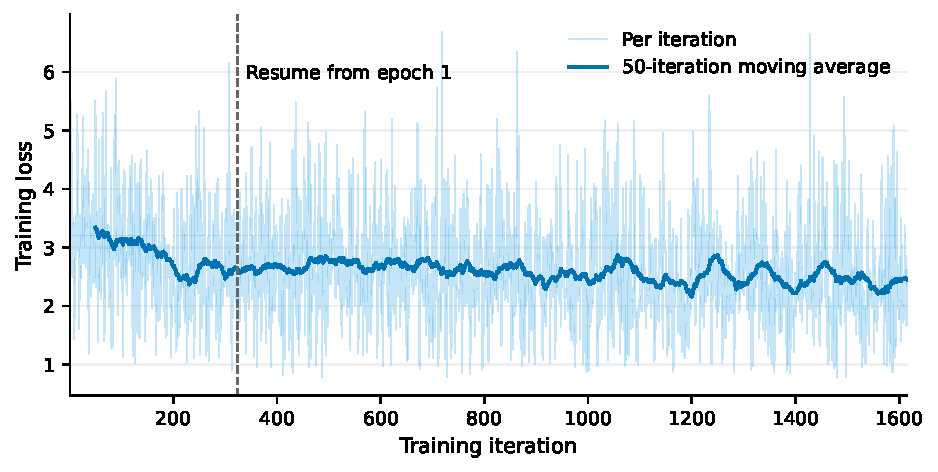
\includegraphics[width=\linewidth]{figures/training_loss.pdf}
  \caption{累计 5 轮训练损失；浅蓝线为逐次损失，深蓝线为 50 次迭代滑动平均，竖虚线为恢复位置}
  \label{fig:loss}
\end{figure}
\FloatBarrier

第 1--5 轮平均损失依次为 2.8699、2.6914、2.5897、2.5064、2.4596。
平均值逐轮下降，单次损失仍有明显波动。曲线记录训练集上的优化过程，验证效果由下面
相同 mini\_val 上的指标判断。

\section{验证结果与 BEV 分析}

\subsection{微调前后的指标}

公开权重测试与最终权重测试的结果分别保存在以 \texttt{baseline} 和
\texttt{finetuned} 结尾的运行目录，\texttt{compare\_results.py} 汇总为
\texttt{outputs/comparison.json}。两次均处理 81 帧，结果见表~\ref{tab:metrics}。

\begin{table}[htbp]
  \centering
  \caption{相同 mini\_val 上的验证结果}
  \label{tab:metrics}
  \begin{tabular}{lrrr}
    \toprule
    指标 & 公开权重基线 & 微调 5 轮 & 变化量 \\
    \midrule
    NDS & 0.026077 & 0.118147 & +0.092070 \\
    mAP & 0.000061 & 0.061377 & +0.061317 \\
    推理及评估时间（s） & 19.139 & 10.521 & --- \\
    \bottomrule
  \end{tabular}
\end{table}

表中计时包含模型构建、推理和评估，不含绘图；两次进程的初始化及缓存状态不同，时间
差值不能用作模型加速结论。微调后 mAP 约为 6.14\%，有提升，但仍然较低。
按类别四个距离阈值的 AP 求平均，car 约为 0.2292、bus 约为 0.3835、pedestrian 约为
0.0011，其余类别为 0；这些分类别数值由框架已四舍五入的距离 AP 汇总，取近似值。
检测能力主要集中在部分车辆，尚不能稳定检出所有类别。

\subsection{同帧对照与误检、漏检}

课程 \texttt{course\_visualization.py} 输出带类别和置信度的预测图，原图只有点云和
预测框。我另外在 \texttt{prepare\_report.py} 中叠加同一 LiDAR 坐标系的真实框，并检查
两次预测顺序与验证索引一致。核对的关键代码如下：

\begin{samepage}
\begin{minted}{python}
for index, sample in enumerate(model_samples):
    meta = sample if isinstance(sample, dict) else sample.metainfo
    assert int(meta['sample_idx']) == int(infos[index]['sample_idx'])
    assert Path(meta['lidar_path']).name == \
        infos[index]['lidar_points']['lidar_path']
\end{minted}
\end{samepage}

图~\ref{fig:before-after} 固定验证清单第 0 帧，两边均使用 0.30 显示阈值。灰点是点云，
蓝色虚线为区域内、有 LiDAR 点的有效类别真实框，橙色实线为预测框，黑色加号为传感器
原点。基线有大量尺寸和位置异常的框；微调后框数从 78 降为 9，但该帧仍有明显误检，
下方两只较大的真实框也没有得到对应预测，不能仅凭框数减少判断检测正确。

\begin{figure}[htbp]
  \centering
  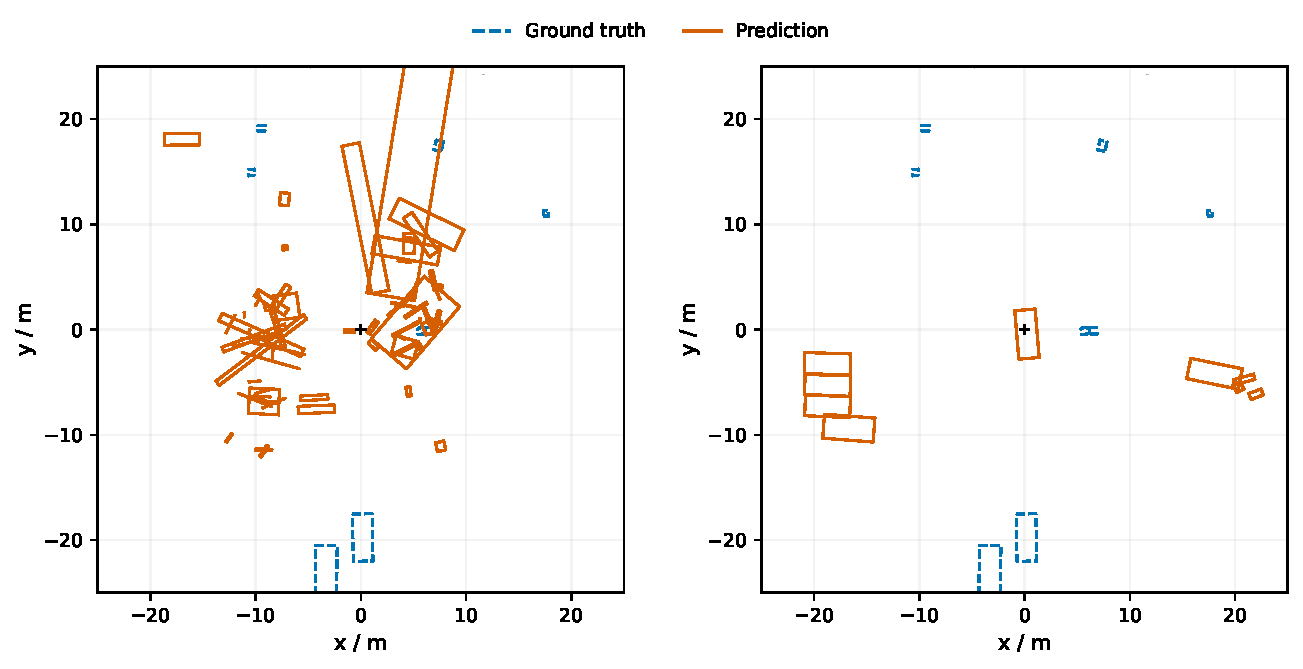
\includegraphics[width=\linewidth]{figures/baseline_vs_finetuned.pdf}
  \caption{验证第 0 帧的同帧对照：左为公开权重，右为微调 5 轮，显示阈值均为 0.30}
  \label{fig:before-after}
\end{figure}
\FloatBarrier

为兼顾两个验证场景，我按清单位置固定选取第 0、40、80 帧，依次来自 scene-0103、
scene-0916、scene-0916，没有按检测分数挑图。图~\ref{fig:fixed} 的中、右图能看到
部分车辆预测贴近真实框，仍有偏离目标的框和未被预测覆盖的真实框。
这些是 BEV 几何对照，图中没有按颜色区分类别，也没有逐框判断官方匹配；指标以
表~\ref{tab:metrics} 的完整评估为准。

\begin{figure}[htbp]
  \centering
  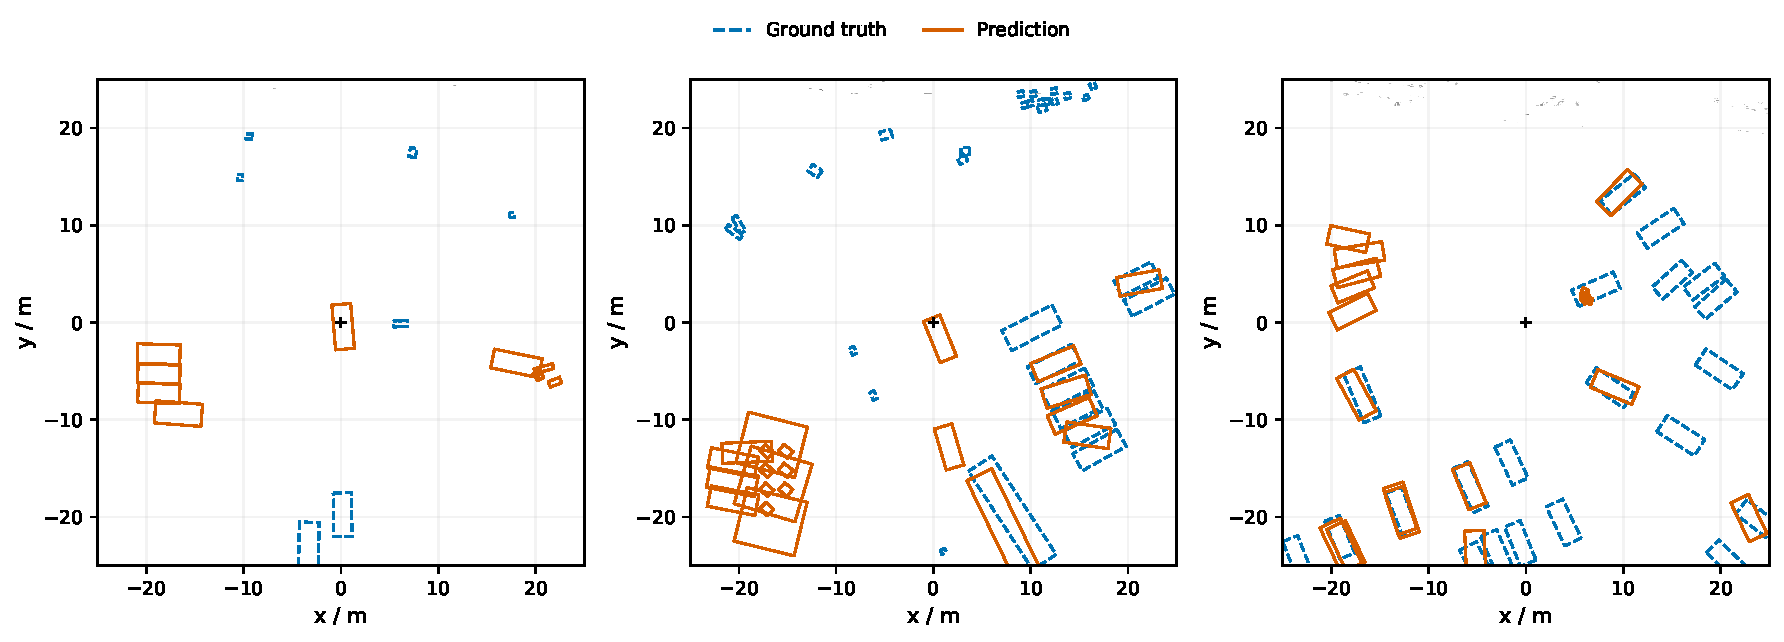
\includegraphics[width=\linewidth]{figures/fixed_samples.pdf}
  \caption{微调后固定第 0、40、80 帧（从左至右），显示阈值 0.30；蓝色虚线是真实框，橙色实线是预测框}
  \label{fig:fixed}
\end{figure}
\FloatBarrier

\subsection{显示阈值的影响}

图~\ref{fig:threshold} 对同一份最终预测重绘，左为 0.10，右为 0.30。
第 0、40、80 帧框数分别从 64/130/71 降至 9/22/19。高阈值去除了很多低分框，图面更
简洁，也可能移除真实目标对应的低分预测。本次只重绘 \texttt{predictions.pkl}，没有
更改模型、内部测试配置或重算评估，NDS 和 mAP 保持原值。

\begin{figure}[htbp]
  \centering
  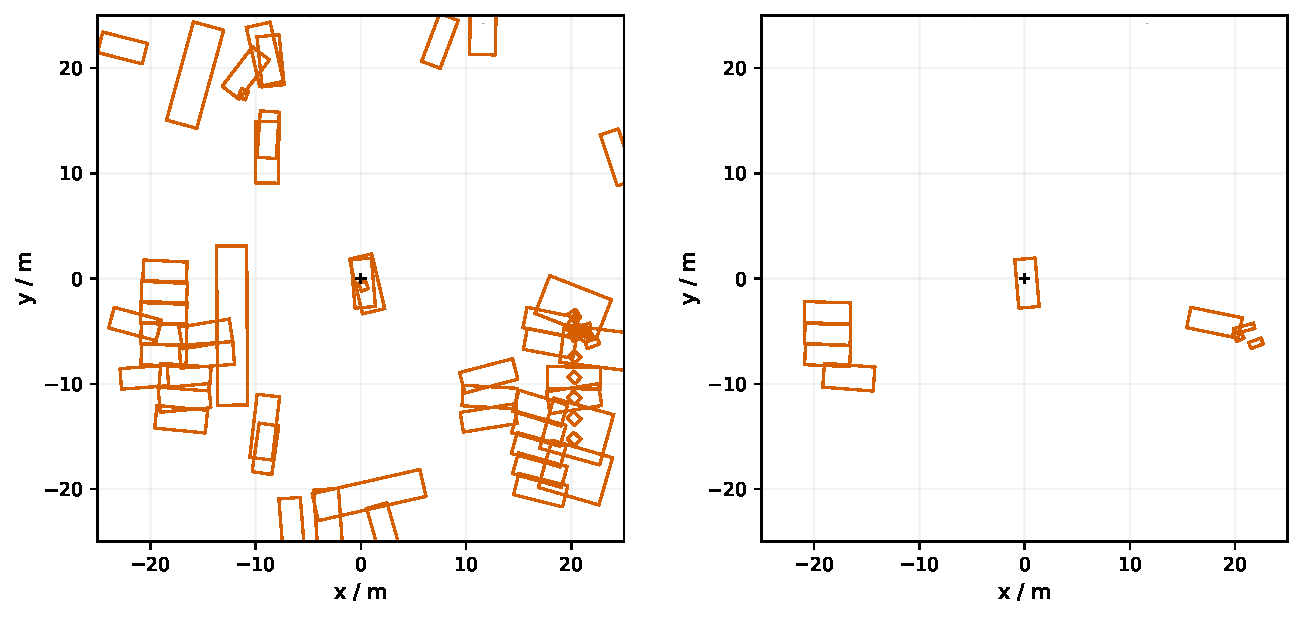
\includegraphics[width=\linewidth]{figures/threshold_comparison.pdf}
  \caption{最终权重在验证第 0 帧的预测：左为 0.10 显示阈值，右为 0.30；此图仅显示预测框}
  \label{fig:threshold}
\end{figure}
\FloatBarrier

\section{实验结果与局限}

本次完成了公开权重基线、1 轮真实微调、断点恢复至累计 5 轮、固定验证和阈值重绘。
训练审计区间合计 87.691 秒；NDS 从 0.026077 升至 0.118147，mAP 从 0.000061 升至
0.061377。与前两次实践相比，这次直接以完整 LiDAR 检测权重初始化，并且只更新检测头
参数，能在小数据集上较快完成实验。

当前仍有明显误检、漏检和类别差异，单帧与 50 m 教学范围也限制了结果的适用范围。
本次没有分别控制输入范围、历史帧或 BatchNorm 运行统计做消融，不能据此确定各因素对
指标的贡献。报告保留了表现较差的第 0 帧及另外两帧对照，并以完整验证集指标记录结果。

\begin{thebibliography}{9}
  \bibitem{pointpillars} A. H. Lang et al., ``PointPillars: Fast Encoders for
  Object Detection from Point Clouds,'' \textit{CVPR}, 2019.
  \bibitem{nuscenes} H. Caesar et al., ``nuScenes: A Multimodal Dataset for
  Autonomous Driving,'' \textit{CVPR}, 2020.
  \bibitem{mmdet3d} OpenMMLab, ``MMDetection3D v1.4.0,''
  \url{https://github.com/open-mmlab/mmdetection3d/tree/v1.4.0}.
\end{thebibliography}

\end{document}
